\chapter{Related Works}

Your related works, and your purpose and contribution which must be different as below.

\section{Aip Suprapto Munari/1164063}
\subsection{Teori}
\subsection{Binary Classification}
\begin{enumerate}
\item Binary Classification atau diartikan kedalam bahasa indonesia yaitu Klasifikasi Biner adalah tugas dalam mengkalrifikasikan elemen-elemen dari himpunan yang diberikan kedalam dua kelompok berdasarkan aturan klarifikasi. Pada ummnya klarifikasi biner akan jatuh ke dalam domain Supervised Learning dan dimana kasus khusus hanya memiliki dua kelas. Beberapa contoh yang meliputi Binary Classification adalah \begin{itemize}
		\item Deteksi Transaksi Penipuan Kartu Kredit
		\item Diagnosa medis
		\item Deteksi Spam
	\end{itemize}
\subitem Untuk contoh Binary Classification dapat dilihat pada gambar \ref{YNBC}
		\begin{figure}[ht]
		\centerline{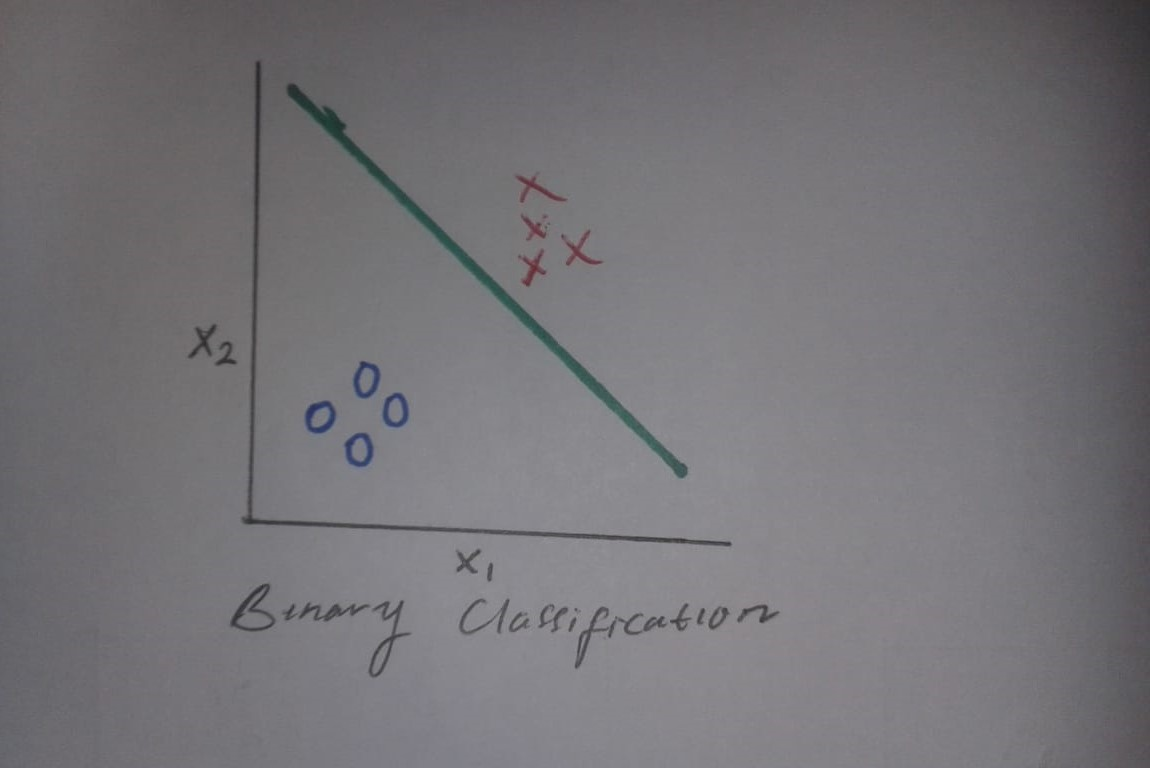
\includegraphics[width=1\textwidth]{figures/AIP/1.JPEG}}
		\caption{Binary Classification.}
		\label{1}
		\end{figure}
 \end{enumerate}

\subsection{Supervised Learning, Unsupervised Learning, Dan Classtering}
\begin{enumerate}
\item Supervised Learning merupakan sebuah pendekatan yang dimana sudah adanya sdata yang dilatih dan telah terdapat variabel yang telah ditargetkan sehingga bertujuan untuk mengelompokkan suatu data ke data yang sudah ada. Contoh dalam Supervised Learning yaitu ketika anda memiliki sejumlah buku yang yang telah dilabel dengan urutan kategori tertentu. Ketika anda akan membeli sebuah buku baru, maka harus di identifikasi isi dari buku tersebut dan memasukkannya kedalam kategori tertentu. Ketika anda membeli sebuah buku tersebut maka anda telah menerapkan sebuah logika fuzzy. Ilustrasi Supervised Learning dapat dilihat pada gambar \ref{YNSL}.

		\begin{figure}[ht]
		\centerline{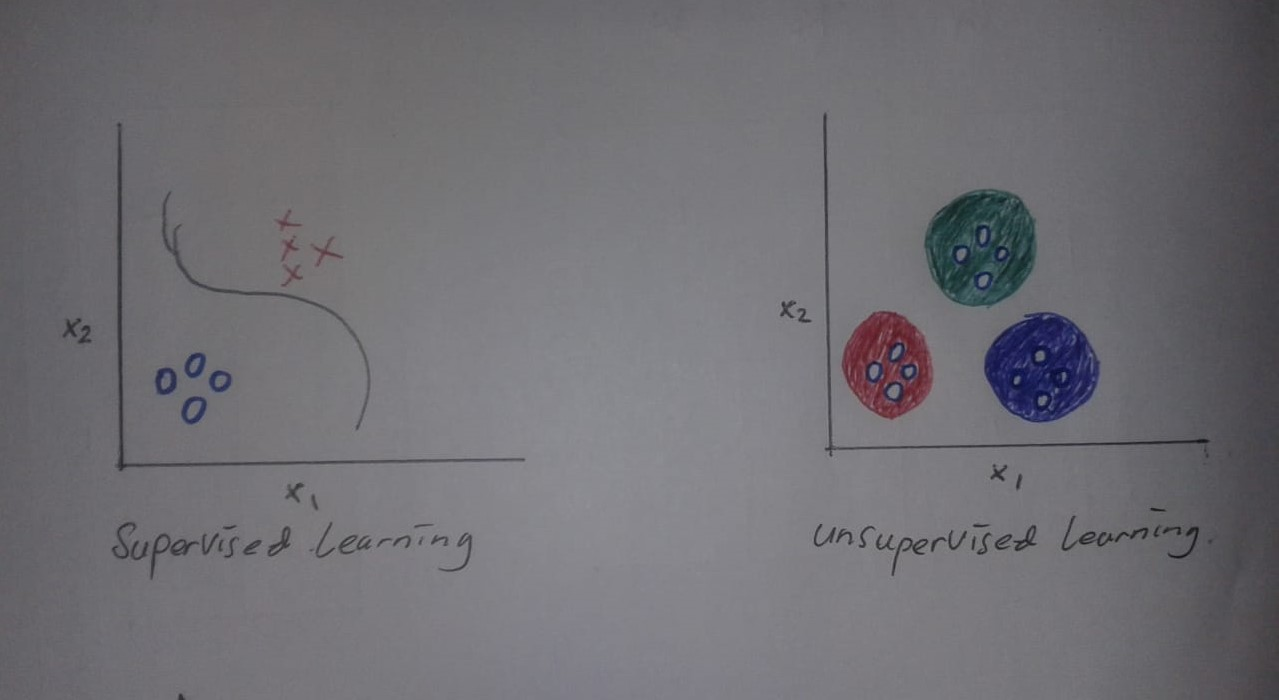
\includegraphics[width=1\textwidth]{figures/AIP/2.JPEG}}
		\caption{Supervised Learning.}
		\label{2}
		\end{figure}

\item Unsupervised Learning merupakan sebuah data yang belum ditentukan variabelnya jadi hanya berupa data saja. Dalam sebuah kasus Unsupervised Learning adalah aggap saja anda belum pernah membeli buku sama sekali dan pada suatu hari anda telah membeli buku dengan sangat banyak dalam kategori yang berbeda. Sehingga buku tersebut belum di kategorikan dan hanya berupa data buku saja. Ilustrasi Unsupervised Learning dapat dilihat pada gambar \ref{YNUSL}.

		\begin{figure}[ht]
		\centerline{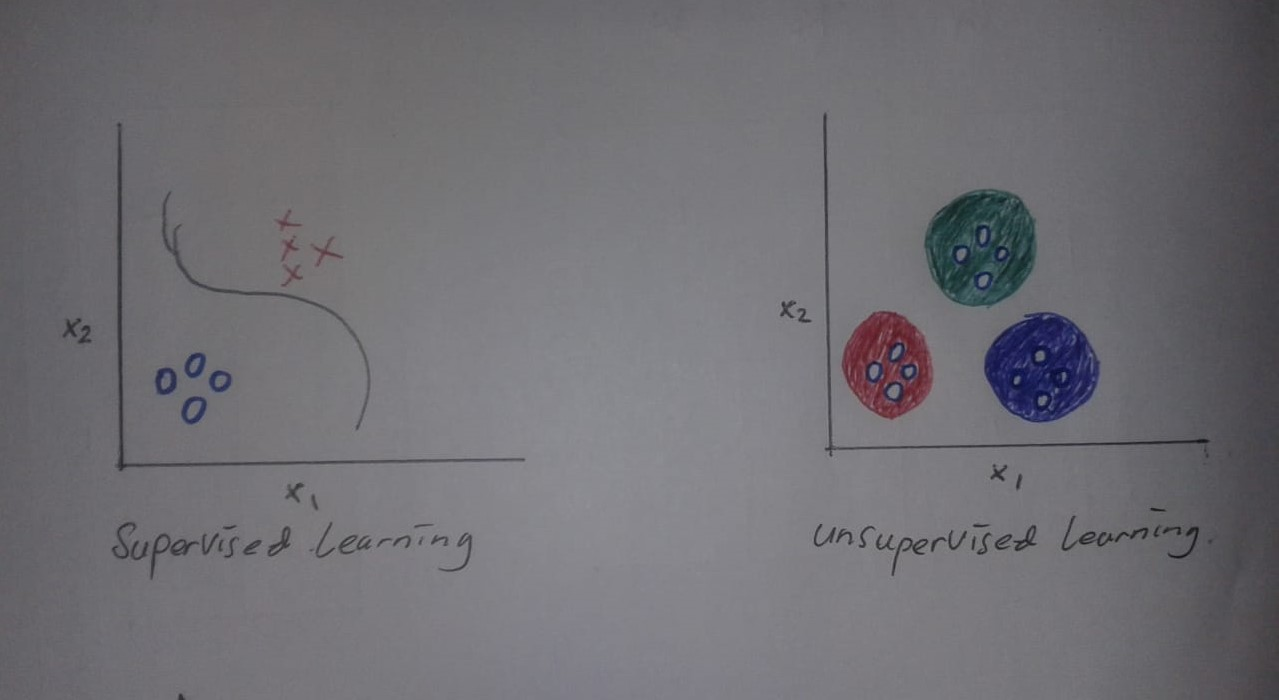
\includegraphics[width=1\textwidth]{figures/AIP/2.JPEG}}
		\caption{Unsupervised Learning.}
		\label{2}
		\end{figure}

\item Classtering merupakan sebuah proses untuk mengklasifikasikan sebuah data dalam satu parameter. Dalam kasus ini dapat dijelaskan ada beberapa orang yang memiliki kekuatan tubuh yang sehat dan kekuatan tubuh yang lemah. Parameter bagi orang yang memiliki tubuh yang kuat adalah orang yang terlihat bugar dan sehat maka dengan orang yang memiliki parameter adalah orang yang memiliki kekuatan tubuh yang kuat dan untuk kekuatan tubuh yang lemah adalah sebaliknya. Ilustrasi gambar dapat di lihat di gambar \ref{YNC}

		\begin{figure}[ht]
		\centerline{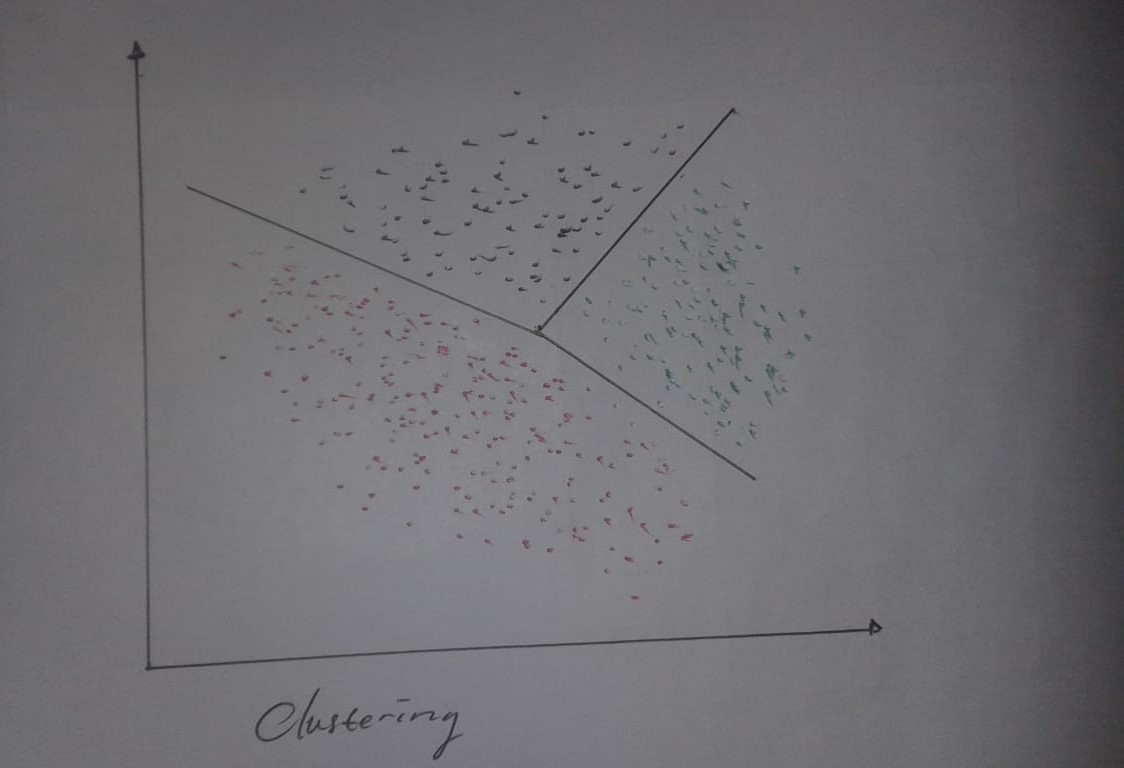
\includegraphics[width=1\textwidth]{figures/AIP/3.JPEG}}
		\caption{Clusterring.}
		\label{3}
		\end{figure}
\end{enumerate}

\subsection{Evaluasi Dan Akurasi}
\begin{enumerate}
\item Evaluasi dan akurasi adalah bagaimana cara kita dapat mengevaluasi sebarapa baik model melakukan pekerjaannya dengan cara mengukur akurasinya. Akurasi akan didefinisikan sebagai presentase kasus yang telah diklasifikasikan dengan benar. Kita dapat melakukan analisis kesalahan yang telah di buat oleh model.Dalam tabel tersebut baris true mangga dan true anggur menunjukkan kasus apakah itu objek mangga atau anggur. Kolom telah di prediksi dan dibuat oleh model. Ada 20 mangga yang di prediksi benar dan ada 5 anggur yang di prediksi salah. Ilustrasi dapat di lihat pada gambar \ref{YEA}

		\begin{figure}[ht]
		\centerline{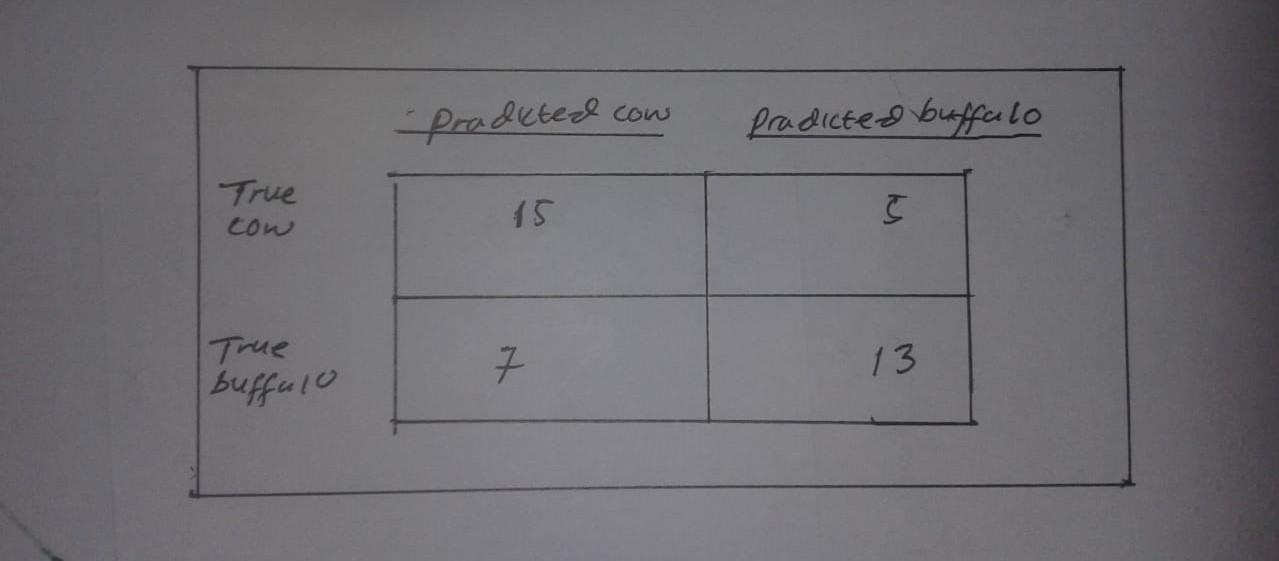
\includegraphics[width=1\textwidth]{figures/AIP/4.JPEG}}
		\caption{Evaluasi Dan Akurasi.}
		\label{4}
		\end{figure}
\end{enumerate}

\subsection{Confusion Matrix}
\begin{enumerate}
\item Ada beberapa cara untuk membuat dan membaca confusion matrix antara lain
	\begin{itemize}
		\item Tentukan pokok permasalahan serta atributnya
		\item Buat Decision Tree
		\item Buat Data Testing
		\item Mencari nilai variabelnya misal a,b,c, dan d
		\item Mencari nilai recall, precision, accuracy, dan erorr rate
	\end{itemize}
\subitem Di bawah ini adalah contoh dari confusion matrix
	\begin{verbatim}
		Recall =3/(1+3) = 0,75
		Precision = 3/(1+3) = 0,75
		Accuracy =(5+3)/(5+1+1+3) = 0,8
		Error Rate =(1+1)/(5+1+1+3) = 0,2 
	\end{verbatim}
\end{enumerate}

\subsection{Cara Kerja K-Fold Cross Validation}
\begin{enumerate}
\item Untuk cara kerja K-Fold Cross Validation adalah sebagai berikut
	\begin{itemize}
		\item Total instance dibagi menjadi N bagian.
		\item Fold yang pertama adalah bagian pertama menjadii testing data dan sisanya menjadi training data.
		\item Hitung akurasi berdasarkan porsi data tersebut dengan menggunakan persamaan.
		\item Fold yang ke dua adalah bagian ke dua menjadi testing data dan sisanya training data. 
		\item Hitung akurasi berdasarkan porsi data tersebut.
		\item Lakukan step secara berulang hingga habis mencapai fold ke-K.
		\item Terakhir hitung rata-rata akurasi K buah.
	\end{itemize}

\subitem Untuk ilustrasi K-Fold Cross Validation data di lihat pada gambar \ref{YNKF}
		\begin{figure}[ht]
		\centerline{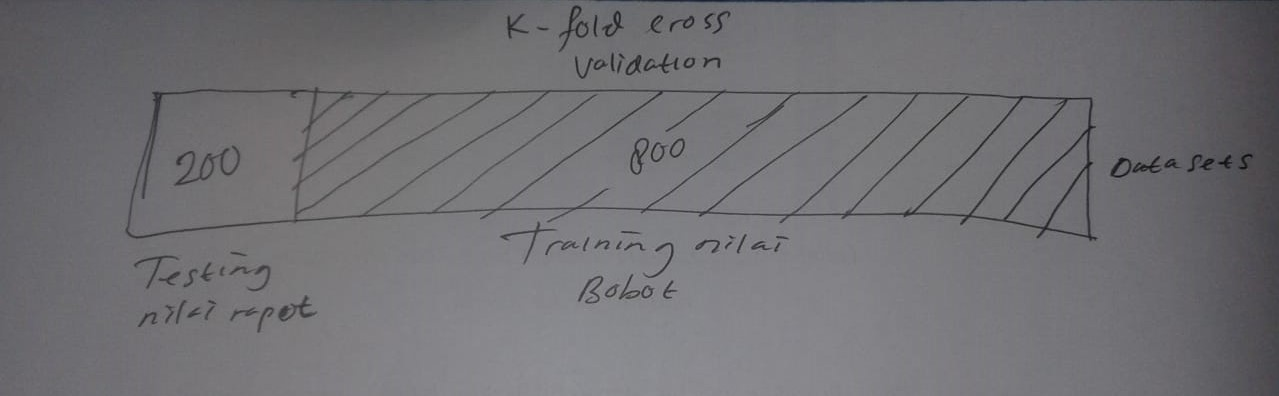
\includegraphics[width=1\textwidth]{figures/AIP/5.JPEG}}
		\caption{K-Fold Cross Validation.}
		\label{5}
		\end{figure}
\end{enumerate}

\subsection{Decision Tree}
\begin{enumerate}
\item Decision Tree adalah sebuah metode pembelajaran yang digunakan untuk melakukan klarifikasi dan regresi. Decision Tree digunakan untuk membuat sebuah model yang dapat memprediksi sebuah nilai variabel target dengan cara mempelajari aturan keputusan dari fitur data. Contoh Decision Tree adalah untuk melakukan predikisi apakah Kuda termasuk hewan mamalia atau bukan, lihat pada gambar \ref{YNDT}.

		\begin{figure}[ht]
		\centerline{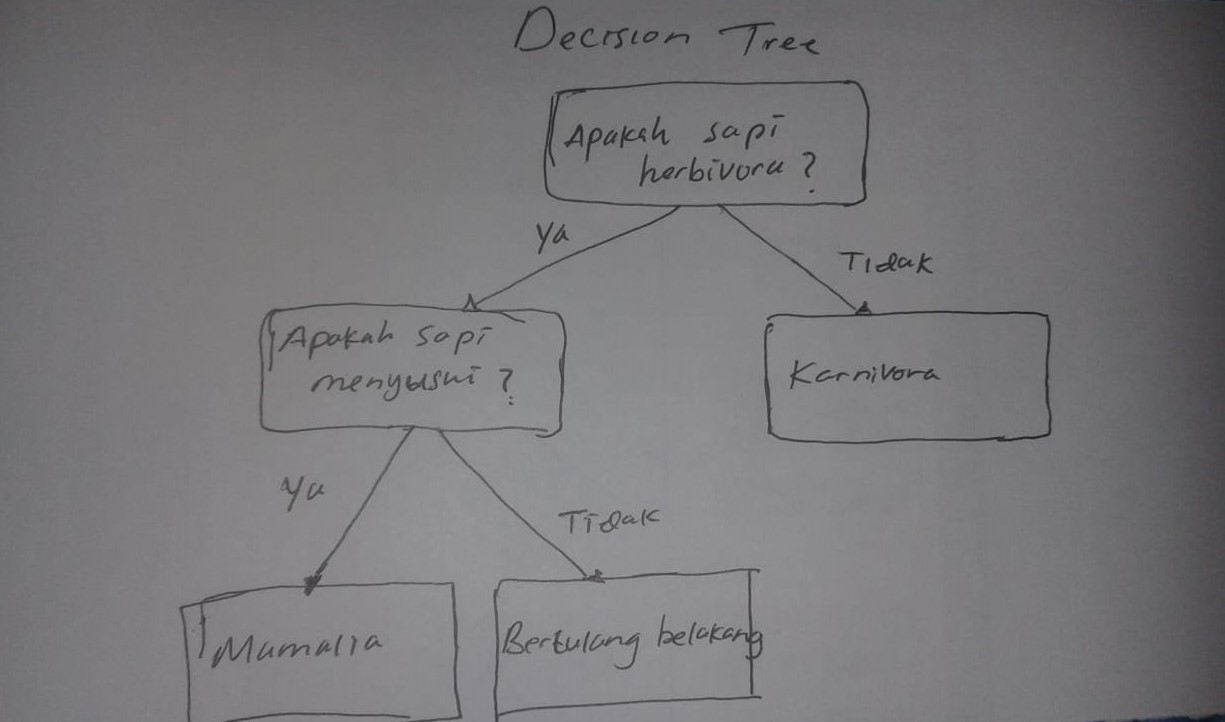
\includegraphics[width=1\textwidth]{figures/AIP/6.JPEG}}
		\caption{Decision Tree.}
		\label{6}
		\end{figure}

\end{enumerate}

\subsection{Gain Dan Entropi}
\begin{enumerate}
\item Gain adalah pengurangan yang diharapkan dalam enthropy. Dalam mechine learning, gain dapat digunakan untuk menentukan sebuah urutan atribut atau memperkecil atribut yang telah dipilih. Urutan ini akan membentuk decision tree. atribut gain dipilih yang paling besar.

\item Entropi adalah ukuran ketidakpastian sebuah variabel acak sehingga dapat di artikan entropi adalah ukuran ketidakpastian dari sebuah atribut.

\subitem Ilustrasi dari gain dan entropi adalah bagaimana kita memprediksi jenis kelamin berdasarkan atributnya, perhatikan pada gambar \ref{YNGE}

		\begin{figure}[ht]
		\centerline{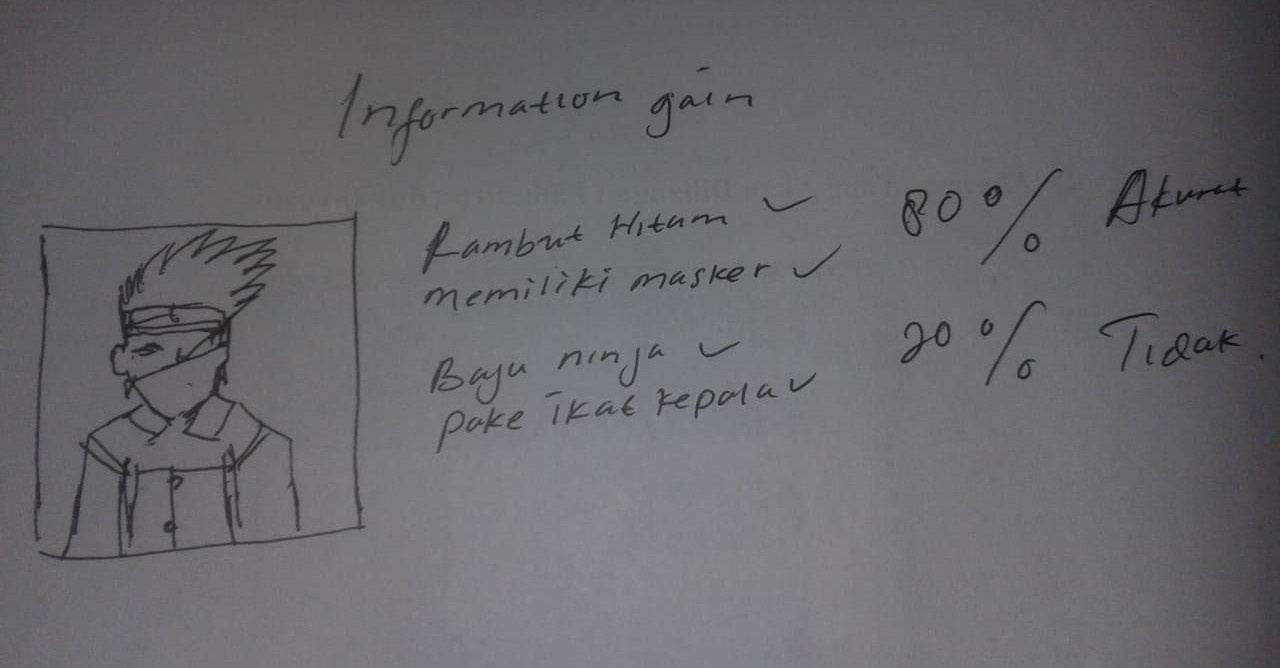
\includegraphics[width=1\textwidth]{figures/AIP/7.JPEG}}
		\caption{Gain Dan Entropi.}
		\label{7}
		\end{figure}
\end{enumerate}

\section{Andi Aslam/1164064}
\subsection{Binary Clasification beserta gambar}
\begin{enumerate}
\item Output aktual dari banyak algoritma klasifikasi biner adalah skor prediksi. Skor menunjukkan kepastian sistem bahwa pengamatan yang diberikan adalah milik kelas positif. Untuk membuat keputusan tentang apakah pengamatan harus diklasifikasikan sebagai positif atau negatif, sebagai konsumen skor ini, Anda akan menginterpretasikan skor dengan memilih ambang klasifikasi (cut-off) dan membandingkan skor dengan itu. Setiap pengamatan dengan skor lebih tinggi dari ambang kemudian diprediksi sebagai kelas positif dan skor lebih rendah dari ambang diprediksi sebagai kelas negatif.

\begin{figure}[ht]
\centering
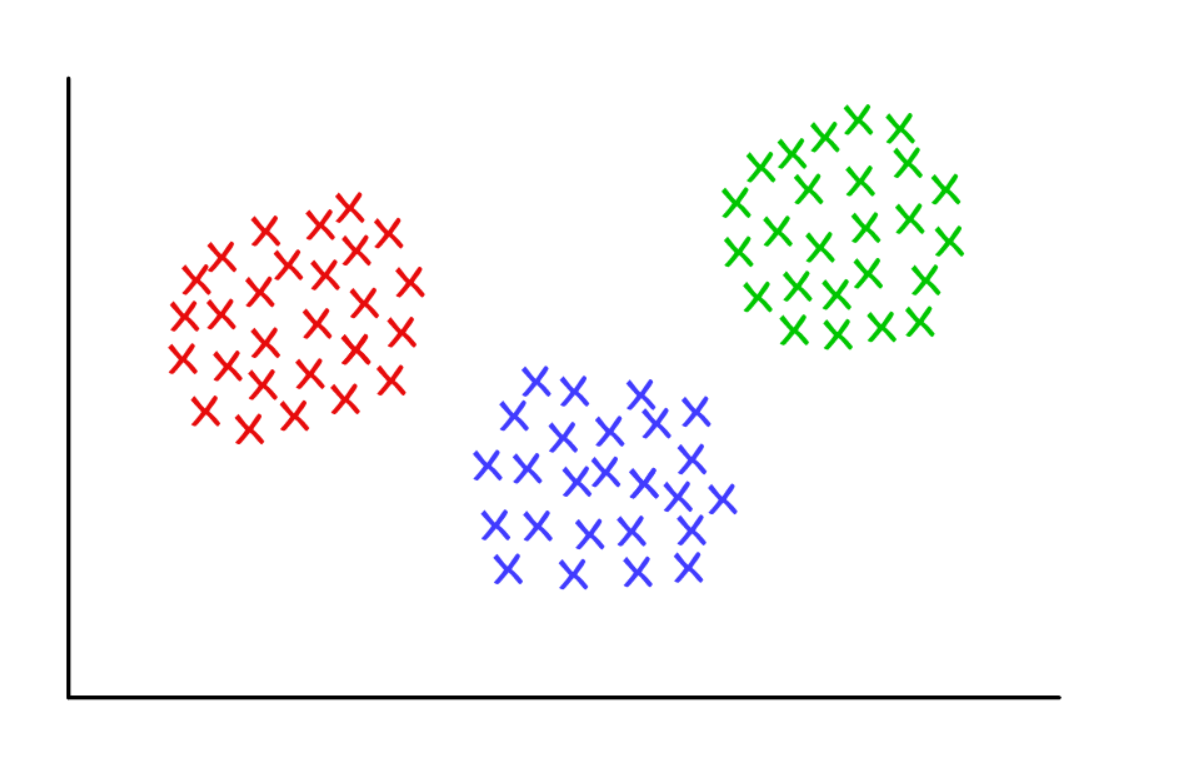
\includegraphics[scale=0.5]{figures/andi/clustring1.png}
\caption{Binary Clasification}
\label{contoh}
\end{figure}
\end{enumerate}

\subsection{supervised learning dan unsupervised learning dan clustering dengan ilustrasi gambar}
\begin{enumerate}
\item Supervised learning adalah tugas pembelajaran mesin untuk mempelajari suatu fungsi yang memetakan input ke output berdasarkan contoh pasangan input-output. Ini menyimpulkan fungsi dari data pelatihan berlabel yang terdiri dari serangkaian contoh pelatihan. Dalam pembelajaran yang diawasi, setiap contoh adalah pasangan yang terdiri dari objek input (biasanya vektor) dan nilai output yang diinginkan (juga disebut sinyal pengawas). Algoritma pembelajaran yang diawasi menganalisis data pelatihan dan menghasilkan fungsi yang disimpulkan, yang dapat digunakan untuk memetakan contoh-contoh baru. Skenario optimal akan memungkinkan algoritma menentukan label kelas dengan benar untuk instance yang tidak terlihat. Ini membutuhkan algoritma pembelajaran untuk menggeneralisasi dari data pelatihan untuk situasi yang tidak terlihat dengan cara yang "masuk akal" (lihat bias induktif).
\item Unsupervised learning adalah istilah yang digunakan untuk pembelajaran bahasa Ibrani, yang terkait dengan pembelajaran tanpa guru, juga dikenal sebagai organisasi mandiri dan metode pemodelan kepadatan probabilitas input. Analisis cluster sebagai cabang pembelajaran mesin yang mengelompokkan data yang belum diberi label, diklasifikasikan atau dikategorikan. Alih-alih menanggapi umpan balik, analisis klaster mengidentifikasi kesamaan dalam data dan bereaksi berdasarkan ada tidaknya kesamaan di setiap potongan data baru. BErikut merupakan contoh Unsupervised Learning dengan Gaussian mixture models.


\begin{figure}[ht]
\centering
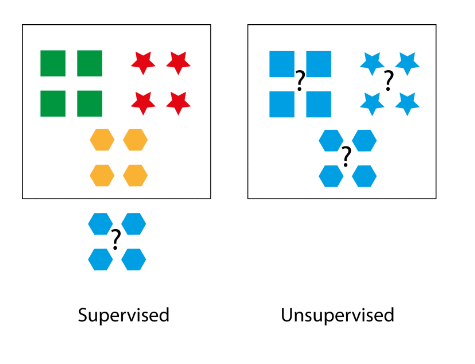
\includegraphics[scale=1]{figures/andi/ilustrasi2.PNG}
\caption{Supervised Learning}
\label{ilustrasi gambar}
\end{figure}
\end{enumerate}

\subsection{evaluasi dan akurasi dari buku dan disertai ilustrasi contoh dengan gambar}
\begin{enumerate}
\item Evaluasi adalah tentang  bagaimana kita dapat mengevaluasi seberapa baik model bekerja dengan mengukur akurasinya. Dan akurasi akan didefinisikan sebagai persentase kasus yang diklasifikasikan dengan benar. Kita dapat menganalisis kesalahan yang dibuat oleh model, atau tingkat kebingungannya, menggunakan matriks kebingungan. Matriks kebingungan mengacu pada kebingungan dalam model, tetapi matriks kebingungan ini bisa menjadi sedikit sulit untuk dipahami ketika mereka menjadi sangat besar.
\begin{figure}[ht]
\centering
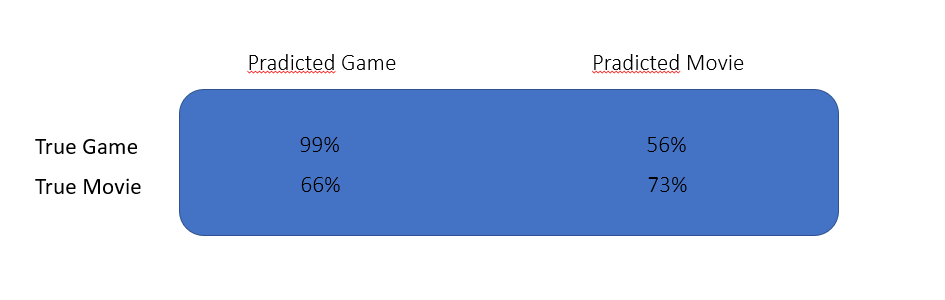
\includegraphics[scale=1]{figures/andi/no3.PNG}
\caption{ Evaluasi dan Akurasi}
\label{contoh}
\end{figure}
\end{enumerate}

\subsection{ bagaimana cara membuat dan membaca confusion matrix, buat confusion matrix }
\begin{enumerate}
\item  Confusion matrix :
\begin{itemize}
\item 1)	Tentukan pokok permasalahan dan atributanya, misal gaji dan listik.
\item 2)	Buat pohon keputusan
\item 3)	Lalu data testingnya
\item 4)	Lalu mencari nilai a, b, c, dan d. Semisal a = 5, b = 1, c = 1, dan d = 3.
\item 5)	Selanjutnya mencari nilai recall, precision, accuracy, serta dan error rate.
\end{itemize}
\item Berikut adalah contoh dari confusion matrix :
\begin{itemize}
\item Recall =3/(1+3) = 0,75
\item Precision = 3/(1+3) = 0,75
\item Accuracy =(5+3)/(5+1+1+3) = 0,8
\item Error Rate =(1+1)/(5+1+1+3) = 0,2
\end{itemize}
\end{enumerate}

\subsection{bagaimana K-fold cross validation bekerja dengan gambar ilustrasi}
\begin{enumerate}
\item Cara kerja K-fold cross validation :
\begin{itemize}
\item 1)	Total instance dibagi menjadi N bagian.
\item 2)	Fold yang pertama adalah bagian pertama menjadi data uji (testing data) dan sisanya menjadi training data.
\item 3)	Lalu hitung akurasi berdasarkan porsi data tersebut dengan menggunakan persamaan.
\item 4)	Fold yang ke dua adalah bagian ke dua menjadi data uji (testing data) dan sisanya training data. 
\item 5)	Kemudian hitung akurasi berdasarkan porsi data tersebut.
\item 6)	Dan seterusnya hingga habis mencapai fold ke-K.
\item 7)	Terakhir hitung rata-rata akurasi K buah.
\end{itemize}
\begin{figure}[ht]
\centering
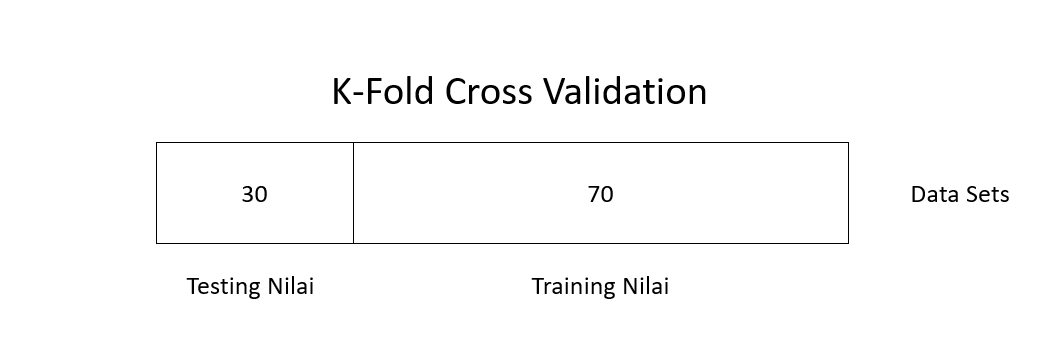
\includegraphics[scale=1]{figures/andi/no5.PNG}
\caption{K-fold cross validation}
\label{contoh}
\end{figure}
\end{enumerate}

\subsection{decision tree dengan gambar ilustrasi}
\begin{enumerate}
\item Decision Tree dalah metode pembelajaran yang diawasi non-parametrik yang digunakan untuk klasifikasi dan regresi. Tujuannya adalah untuk membuat model yang memprediksi nilai variabel target dengan mempelajari aturan keputusan sederhana yang disimpulkan dari fitur data.\\
Misalnya, dalam contoh di bawah ini, decision tree belajar dari data untuk memperkirakan kurva sinus dengan seperangkat aturan keputusan if-then-else. Semakin dalam pohon, semakin rumit aturan keputusan dan semakin bugar modelnya.
\begin{figure}[ht]
\centering
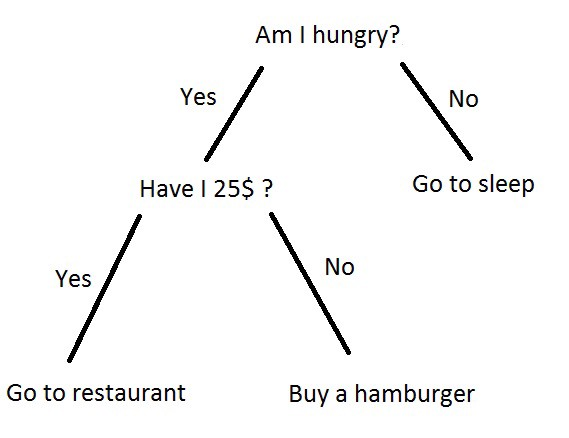
\includegraphics[scale=0.5]{figures/andi/tree.jpg}
\caption{Decision Tree}
\label{contoh}
\end{figure}
\end{enumerate}

\subsection{Information Gain dan entropi dengan gambar ilustrasi}
\begin{enumerate}
\item Information gain didasarkan pada penurunan entropi setelah dataset dibagi pada atribut. Membangun decision tree adalah semua tentang menemukan atribut yang mengembalikan perolehan informasi tertinggi (mis., Cabang yang paling homogen).
\item Entropi adalah ukuran keacakan dalam informasi yang sedang diproses. Semakin tinggi entropi, semakin sulit untuk menarik kesimpulan dari informasi itu. Membalik koin adalah contoh tindakan yang memberikan informasi yang acak. Untuk koin yang tidak memiliki afinitas untuk kepala atau ekor, hasil dari sejumlah lemparan sulit diprediksi. Mengapa? Karena tidak ada hubungan antara membalik dan hasilnya. Inilah inti dari entropi.
\begin{figure}[ht]
\centering
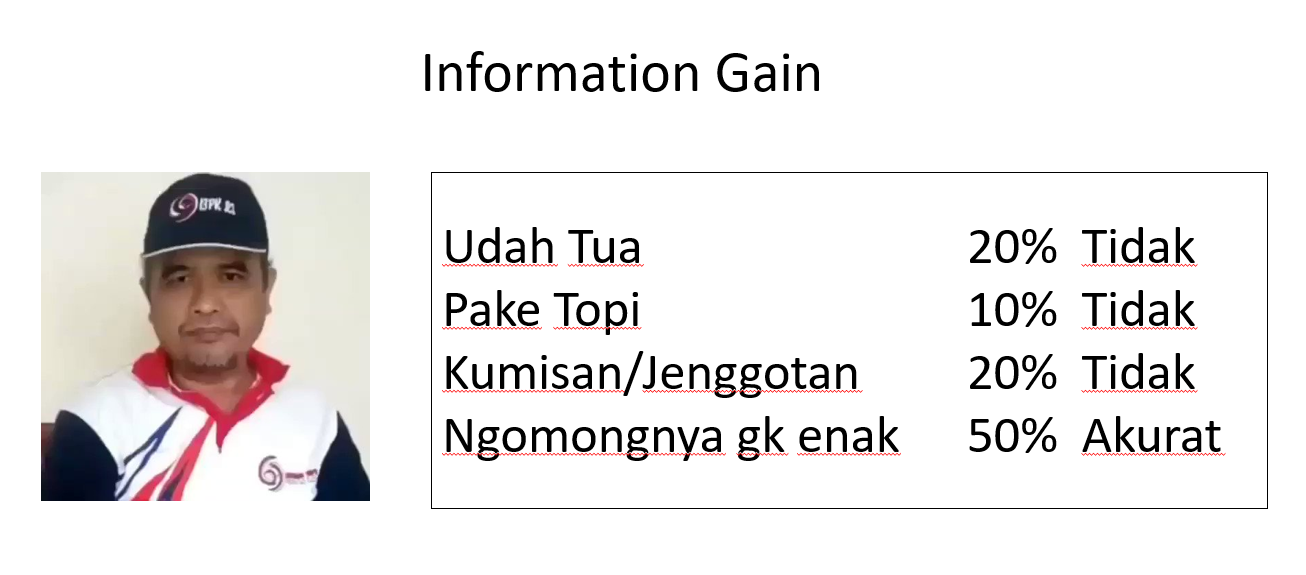
\includegraphics[scale=0.5]{figures/andi/no7.PNG}
\caption{Entropi}
\label{contoh}
\end{figure}
\end{enumerate}


\section{Same Topics}
Cite every latest journal with same topic
\subsection{Topic 1}
cite for first topic

\subsection{Topic 2}
if you have two topics you can include here to


\section{Same Method}
write and cite latest journal with same method

\subsection{Method 1}
cite and paraphrase method 1

\subsection{Method 2}
cite and paraphrase method 2 if you have more method please add new subsection.




 